
\chapter[Augmented Gromov-Wasserstein]{Augmented Gromov-Wasserstein}

\localtableofcontents*

\chaptermark{\textbf{Augmented Gromov-Wasserstein}}

Gromov-Wasserstein distance has many applications in machine learning due to its ability
to compare measures across metric spaces and its invariance to isometric transformations. However,
in certain applications, this invariant property can be too flexible, thus undesirable. Moreover,
the Gromov-Wasserstein distance solely considers pairwise sample similarities in input datasets,
disregarding the raw feature representations. We propose a new optimal transport formulation,
called Augmented Gromov-Wasserstein (AGW), that allows for some control over the
level of rigidity to transformations. It also incorporates feature alignments,
enabling us to better leverage prior knowledge on the input data for improved performance.
We present theoretical insights into the proposed method. We then demonstrate its usefulness
for single-cell multi-omic alignment tasks and heterogeneous domain adaptation in machine learning.

\section{Introduction}

Optimal transport (OT) theory provides a fundamental tool for comparing and
aligning probability measures omnipresent in machine learning (ML) tasks.
Following the least effort principle, OT and its associated metrics offer
many attractive properties that other divergences, such as the popular Kullback-Leibler or
Jensen-Shannon divergences, lack. For instance, OT borrows key geometric properties of
the underlying ``ground'' space on which the distributions are defined \citep{Villani03}
and enjoys non-vanishing gradients when measures have disjoint support \citep{Arjovsky17}.
OT theory has also been extended to a much more challenging case of probability measures supported
on different metric-measure spaces. In this scenario, the Gromov-Wasserstein (GW) distance
seeks an optimal matching between points in the supports of the considered distributions
that will minimize the distortion of intra-domain distances upon such matching.

Since its proposal by \citep{Memoli11} and further extensions by \citep{Peyre16},
GW has been successfully used in a wide range of applications, including
domain adaptation \citep{Yan18}, computational biology
\citep{Nitzan2019,Pamona,UniPort,SpaOTsc,Demetci20,Demetci22,PASTE},
generative modeling \citep{Bunne19}, and reinforcement learning \citep{GW-VAE}.

\paragraph{Limitations of prior work} Successful applications of GW distance are often attributed to its invariance to distance-preserving transformations (also called ``isometries'') of the input domains. Since GW considers only intra-domain distances, it is naturally invariant to any transformation that does not alter them. While this is a blessing in many applications, for example, comparing graphs with the unknown ordering of nodes, it may become a curse when one has to choose the ``right'' isometry among many that yield the same GW distance. How could one break such ties while keeping the attractive properties of the GW distance? This question remains to be addressed in the field.

Additionally, GW distances are often used in tasks where one may have some
\textit{a priori} knowledge about the mapping between the two considered spaces.
For example, in single-cell applications, mapping a group of cells in similar tissues
across species helps understand the evolutionarily conserved and diverging cell types
and functions \citep{kriebel2022uinmf}. When performed using OT, this cross-species cell mapping
may benefit from the knowledge about an overlapping set of orthologous genes
\footnote {Genes in two different species that originated from a common ancestor and
largely maintained their function and sequence during speciation}.
GW formulation does not offer any straightforward way to incorporate this knowledge,
which may lead to suboptimal performance.

\paragraph{Our contributions}
In this paper, we introduce a new OT formulation that addresses the drawbacks of the
GW distance mentioned above. We summarize our contributions as follows:
\begin{enumerate}
    \item We propose Augmented Gromov-Wasserstein (AGW), a new formulation that leverages
    both pairwise sample similarities in input datasets and their raw data representations;
    \item We demonstrate that AGW allows for better control over the isometric transformations
    of the GW distance and helps break isometric ties;
    \item We show that AGW can incorporate prior knowledge to guide how the two metric spaces
    should be compared, which improves object comparisons; %object matchings; Priors can also be set to further tighten isometric invariances
    \item We provide a theoretical analysis of the properties of the proposed formulation
    and examples that concretely illustrate its unique features;
    \item Our empirical results show that AGW outperforms previously proposed
    cross-domain OT methods in several downstream tasks and tends to converge in fewer iterations
    than GW. We first focus on real-world applications in computational biology,
    namely the single-cell data integration tasks. Then, we also illustrate its generalizability
    to the heterogeneous domain adaptation in ML.
    %\item runtime
\end{enumerate}
The paper is organized as follows. Section 2 presents key notions from the OT theory
utilized in the rest of the paper. Section 3 presents our proposed AGW formulation and
analyzes its theoretical properties. In Section 4, we present several empirical studies
for the single-cell alignment task and demonstrate the applicability of our method to
the heterogeneous domain adaptation task. We conclude our paper in Section 5 with
a discussion of potential future work.

\paragraph{Notations} In what follows, we denote by
$Delta_{n}=\{w \in (\bbR_{+})^{n}:\ \sum_{i=1}^{n} w_{i}=1\}$
the simplex histogram with $n$ bins. We use $\otimes$ for tensor-matrix multiplication,
\ie $L \otimes B$ is the matrix $(\sum_{k,l} L_{i,j,k,l} B_{k,l})_{i,j}$ for a tensor
$L =(L_{i,j,k,l})_{i,j,k,l}$ and a matrix $B = (B_{i,j})_{i,j}$.
We use $\langle \cdot, \cdot \rangle$ for the matrix scalar product associated with
the Frobenius norm $\|\cdot\|_{F}$. We write $1_d \in \bbR^d$ for a
$d$-dimensional vector of ones.
We use the terms ``coupling matrix'', ``transport plan'' and ``correspondence matrix'' interchangeably.
A point in the space can also be called ``an example'' or ``a sample''.
Given an integer $n \geq 1$, denote $[n] := \{ 1, ..., n\}$.

%%%%%%%%%%%%%%%%%%%%%%%%%%%%%%%%%%%%%%%%%%%%%%%%%%%%%%%%%%%%%%%%
\section{Technical background}

This section briefly presents some background knowledge,
including the Kantorovich formulation of the OT problem and two relevant OT-based distances
proposed to match samples across incomparable spaces.

\paragraph{Kantrovich OT and Wasserstein distance}
Let $X \in \bbR^{n\times d}$ and $Y \in \bbR^{m\times d}$ be two input matrices,
$C \in \bbR^{m \times n}$ be a cost (or ground) matrix.
Given two discrete probability measures $\mu \in Delta_n$ and $\nu\in Delta_m$,
Kantorovich formulation of OT seeks a coupling $P$ minimizing the following quantity:
\begin{equation}
  W_C(\mu,\nu) = \min_{P \in U(\mu,\nu)} \langle C, P \rangle,
  \label{eq:wasserstein}
 \end{equation}
where $U(\mu,\nu)$ is the space of probability distributions over
$\bbR^2$ with marginals $\mu$ and $\nu$. When $C_{ij} = ||x_i - y_j||^p$, for $p \geq 1$,
such an optimization problem defines a proper metric on the space of
probability distributions called the Wasserstein distance.

\paragraph{Gromov-Wasserstein distance}
Samples of input matrices in different spaces, \ie, $X \in \bbR^{n\times d}$
and $Y \in \bbR^{m\times d'}$ with $d \neq d'$, are incomparable since
it is not possible to define a cost function $c$ as the distance between points across
the input spaces.
To circumvent this limitation of the Wasserstein distance, \citep{Memoli11}
proposed the Gromov-Wasserstein (GW) distance, defined as follows:
\begin{align}
% \label{eq:gw}
    \gw(X, Y, \mu, \nu, d_X, d_Y) := \min_{P \in U(\mu, \nu)} L_{\gw} (P),
\end{align}
where
\begin{align*}
\label{eq:gw_func}
    L_{\gw} (P) &:=
    \sum_{i,j,k,l} \big( d_X(x_i,x_k) - d_Y(y_j,y_l) \big)^2 P_{i,j}P_{k,l}
    = \langle L(D_X, D_Y) \otimes P, P \rangle.
\end{align*}
Here, $\big( L(D_X, D_Y) \big)_{i,j,k,l} = \big( d_X(x_i,x_k) - d_Y(y_j,y_l) \big)^2$,
where $(x_i, x_k) \in \bbR^d \times \bbR^d$ and $(y_j, y_k) \in \bbR^{d'} \times \bbR^{d'}$
are tuples of samples in $X$ and $Y$, respectively.
$d_X$ and $d_Y$ are divergences so that $(D_X)_{i,k} = d_X(x_i,x_k)$ and
$(D_Y)_{j,l} = d_Y(y_j,y_l)$.

\paragraph{CO-Optimal transport}
\citep{Redko20} introduced an alternative to GW distance, termed CO-Optimal transport (COOT),
that rather than relying on the intra-domain distance matrices $D_X$ and $D_Y$,
instead takes into account the raw feature information
(\textit{i.e.} the coordinates of the samples) and jointly learns two couplings,
corresponding to the sample and feature alignments. More precisely,
COOT assigns two histograms $\mu' \in Delta_d$ and $\nu' \in Delta_{d'}$ to the
features (columns) of $X$ and $Y$, respectively, and defines the distance between two matrices
$X$ and $Y$ as
\begin{equation*}
  \label{eq:co-optimal-transport}
 \begin{split}
     \coot(X, Y, \mu, \nu, \mu', \nu') :=
     \min_{\substack{P^s \in U(\mu,\nu) \\ P^v \in U(\mu',\nu')}} L_{\coot} (P^s, P^v).
    \end{split}
 \end{equation*}
where
\begin{align*}
    L_\coot (P^s, P^v) &:=  \sum_{i,j,k,l} L(x_{ik},y_{jl})P^s_{i,j} P^v_{k,l}
    =\langle L(X,Y) \otimes P^v,  P^s \rangle.
\end{align*}
In what follows, we consider $L(x_{ik}, y_{jl}) = (x_{ik} - y_{jl})^2$ and write simply
$\gw(X, Y)$ and $\coot(X, Y)$ when $\mu, \nu, \mu', \nu'$
are uniform and when the choice of $d_X$ and $d_Y$ is of no importance.

%%%%%%%%%%%%%%%%%%%%%%%%%%%%%%%%%%%%%%%%%%%%%%%
\section{Augmented Gromov-Wasserstein}

\begin{figure}[t]
\centering
\includegraphics[width=\linewidth]{./Chapitre5/fig//mnist1_supervised.png}
\caption{Aligning digits from MNIST and USPS datasets. \textbf{(A)}
Confusion matrices of GW, AGW with $\alpha=0.5$ and COOT.
(*) denote pair alignments ;
\textbf{(B)} Feature coupling $P^v$ of AGW compared to COOT;
\textbf{(C)} Illustration of a case from where GW's and COOT's invariants are
detrimental for obtaining a meaningful comparison, while AGW remains informative.
\textbf{(D)} Example showing improved digit alignment with feature-level supervision
that restricts reflections \textbf{(E)} Feature coupling recovered by AGW ($\alpha =0.5$)
in the supervised setting of (D).}
\label{fig:mnist}
\end{figure}

Here, we start by outlining the motivation for our proposed formulation,
highlighting the different properties of GW distance and COOT. Then,
we detail our AGW method that interpolates between the two, followed by a
theoretical study of its properties.

\subsection{Motivation}

\paragraph{Invariants of GW} GW distance remains unchanged under isometric transformations of
the input data. This property has contributed much to the popularity of GW distance,
as isometries naturally appear in many applications. However,
not all isometries are equally desirable. For instance, a rotation of the
handwritten digit $6$ seen as a discrete measure can lead to its slight variation
for small angles or to a digit $9$ when the angle is close to $180$ degrees. In both cases,
however, the GW distance remains unchanged, making it insufficient to distinguish
the two digits apart.

\paragraph{Invariants of COOT} Unlike GW, COOT has fewer degrees of freedom
in terms of invariance to global isometric transformations as it is limited to
permutations of rows and columns of the two matrices, and not all isometric transformations
can be achieved via such permutations. For example, Figure S1 shows the effect of the sign change
and image rotation in a handwritten digit matching task, to which GW is invariant while COOT is not.

Additionally, COOT is strictly positive for any two datasets of different sizes either
in terms of features or samples, making it much more restrictive than GW.
It thus provides a fine-grained control when comparing complex objects,
yet it lacks the robustness of GW to frequently encountered transformations
between the two datasets. Further, unlike GW, it is invariant to local isometries
that can be achieved via permutations of a subset of features.

\subsection{AGW formulation}
Given the above discussion on the invariants of COOT and GW distance,
interpolating between them will restrict each other's invariants. Additionally,
interpolating with COOT is a natural way to introduce raw feature alignments in GW,
which allows for leveraging priors on them.
We call this interpolation \textbf{Augmented GW} (AGW) and define it as follows:
% \begin{align}
% \label{eq:scootr}
% \agw_{\alpha}(X, Y) &:= \min_{ \scriptsize{\begin{matrix} P^s \inU(\mu,\nu),\\ P^v \in U(\mu',\nu')\end{matrix}}} \alpha L_{\gw} (P^s) \notag \\ & + (1-\alpha) L_{\coot} (P^s, P^v) \notag \\ & =\min_{ \scriptsize{\begin{matrix}P^s \inU(\mu,\nu),\\ P^v \in U(\mu',\nu')\end{matrix}}} \langle \alpha L(D_X,D_Y)\otimes P^s \notag \\ & + (1-\alpha) L(X,Y) \otimes P^v,  P^s \rangle.
% \end{align}
\begin{align}
\label{eq:scootr}
\agw_{\alpha}(X, Y) &:=
\min_{\substack{P^s \in U(\mu,\nu) \\ P^v \in U(\mu',\nu')}} L_{\alpha}(P^s, P^v),
\end{align}
where
\begin{align*}
    L_{\alpha}(P^s, P^v) &= \alpha \; L_{\gw} (P^s) + (1-\alpha) \; L_{\coot} (P^s, P^v) \\
    =& \alpha \; \langle L(D_X,D_Y)\otimes P^s,P^s \rangle \\
    &+ (1-\alpha) \; \langle L(X,Y) \otimes P^v,P^s \rangle
\end{align*}

The AGW problem always admits a solution. Indeed, as the objective function is continuous
and the sets of admissible couplings are compact, the existence of minimum and minimizer
is guaranteed.

Our interpolation offers several important benefits. First, COOT term ensures that AGW
will take different values for any two isometries whenever $d \neq d'$. Intuitively,
AGW's value will then depend on how ``far'' a given isometry is from a permutation of rows
and columns of the inputs. Thus, we restrict a broad class of (infinitely many) transformations
that GW cannot distinguish and we tell them apart by assessing whether they
can be approximately obtained by simply swapping 1D elements in input matrices.
%[can mention local isometries here]

Second, combining the objective functions of COOT and GW distance allows us to
effectively influence the optimization of $P^s$ by introducing priors on feature matchings
through $P^v$ and vice versa. This can be achieved by penalizing the costs of matching
certain features in the COOT term to influence the optimization of $P^v$. This prior knowledge
guides how the two metric spaces should be compared and improves empirical performance.
These key properties explain our choice of calling it ``augmented'':
we equip GW distance with an ability to provide finer-grained object comparisons by
breaking isometric ties and/or guiding the matching using available prior knowledge.

\paragraph{Illustrations} We illustrate $\agw$'s properties on a task of aligning handwritten digits
from MNIST \citep{lecun10} (28$\times$28 pixels) and USPS datasets (16$\times$16 pixels)
\citep{Hull94} in \Cref{fig:mnist}, where AGW with $\alpha=0.5$ outperforms both GW and COOT
in alignment accuracy (Panel A). The black asterisks show the digit pairs that most benefit
from AGW interpolation, which are $6-2$ for GW and $3-5$ for COOT.
Panel C visualizes examples from these digit pairs that are misaligned by GW and COOT
but not by AGW.
\footnote{Here, we define ``aligned pairs'' as pairs of digits with the
highest coupling probabilities.}. Here, we observe that 6-2 misalignment by GW is likely because
one is a close reflection of the other across the y-axis. Similarly,
COOT mismatches 3 and 5 as one can obtain 3 from 5 by a local permutation of
the upper half of the pixels. Panel B visualizes the feature couplings obtained by
AGW (on the left) and COOT (on the right). The feature coupling by COOT confirms that
COOT allows for a reflection across the y-axis on the upper half of the image
but not on the lower half. With AGW, both of these misalignments improve,
likely because (1) the correct feature alignments in the lower half of the images
prevent 6 and 2 from being matched and (2) GW distance is non-zero for 5-3 matches
since the transformation is not applied to the whole image. In Panels D and E,
we also show that providing supervision on feature alignments to restrict local reflections
further improves AGW's performance.

Similar improvement can be seen for aligning cells (samples) for two different single-cell
measurements (features) \citep{SNAREseq} in Figure S2. Panel A shows that AGW consistently maps
the 4 cell types in the data better than GW (a popular method for this task
\citep{Pamona,Demetci20,Demetci22,UniPort}) over 50 random subsampling of cells.
The 2D projection of alignments in Panel B shows that GW sometimes completely swaps
the cell type clusters when they have a similar number of cells, whereas AGW is more robust
to this phenomenon.

\paragraph{Optimization} For simplicity, let $n = m$ and $d = d'$.
With the squared loss in both GW and COOT terms, the computational trick by \citep{Peyre16}
can be applied, which reduces the complexity of $\agw$ from $O(n^4 + n^2 d^2)$
to $O(n^3 + dn^2 + nd^2)$. For optimization, we use the block coordinate descent (BCD) algorithm,
where we alternatively fix one coupling and minimize AGW with respect to the other (\Cref{alg:bcd}).
Each iteration then consists of solving two OT problems. To further accelerate the optimization,
entropic regularization can be used \citep{Cuturi13} on either $P^s$, $P^v$, or both.
In practice, we rely on the built-in functions of the POT package \citep{Flamary21}.

\begin{algorithm}[!t]
    \caption{BCD algorithm to solve AGW \label{alg:bcd}}
    \begin{algorithmic}[t]
      % \STATE {\textbf{Input:}} $\bA \in \bbR^{n_1, d_1}, \bB \in \bbR^{n_2, d_2}$, $\lambda_1, \lambda_2, \varepsilon$
      \STATE Initialize $P^s$ and $P^v$
      \REPEAT
      \STATE Calculate $L_v = L(X, Y) \otimes P^s$.
      \STATE For fixed $P^s$, solve the OT problem:
      $P^v \in \arg\min_{P \in U(\mu', \nu')} \langle L_v, P \rangle$.
      \STATE Calculate $L_s = L(X, Y) \otimes P^v$.
      \STATE For fixed $P^v$, solve the fused GW problem:
      $P^s \in \arg\min_{P \in U(\mu, \nu)} \alpha \; L_{\gw} (P^s)
      + (1-\alpha) \langle L_s, P^s \rangle$.
      \UNTIL{convergence}
\end{algorithmic}
\end{algorithm}

\subsection{Theoretical analysis}

Intuitively, we expect that AGW interpolates between GW and COOT and shares similar properties
with Fused Gromov-Wasserstein (FGW) distance \citep{Vayer19b}, namely
the relaxed triangle inequality (since COOT and GW distances are both metrics).
The following result summarizes these observations, whose proofs are presented in
Appendix.
\begin{proposition}
\label{prop:basic_prop}
For every $\alpha \in [0, 1]$, given two input matrices $X$ and $Y$,
\begin{enumerate}
    \item When $\alpha \to 0$ (or $1$), one has $\agw_{\alpha}(X, Y) \to \coot(X, Y)$ (or $\gw(X, Y)$).

    \item $\agw$ satisfies the relaxed triangle inequality: for any input matrices $X, Y, Z$,
    one has $\agw_{\alpha}(X, Y) \leq 2 \big( \agw_{\alpha}(X, Z) + \agw_{\alpha}(Z, Y) \big)$.
\end{enumerate}
\end{proposition}

% As $\alpha$ tends to zero, the $\agw_{\alpha}(\mathbb X, \mathbb Y)$ approaches $\coot(\mathbb X, \mathbb Y)$ and as $\alpha$ tends to 1, it approaches $\gw\left((X, \mu_{sx}), (Y, \mu_{sy}) \right)$:
% \begin{align*}
%     \lim_{\alpha \rightarrow 0} \text{GWC}_{\alpha}(\hat{\mu}, \hat{\nu}, \hat{\mu'}, \hat{\nu'}) &= \coot(\hat{\mu}, \hat{\nu}, \hat{\mu'}, \hat{\nu'})\\
%     \lim_{\alpha \rightarrow 1} \text{GWC}_{\alpha}(\hat{\mu}, \hat{\nu}, \hat{\mu'}, \hat{\nu'}) &= \gw(\hat{\mu}, \hat{\nu})
% \end{align*}
% These basic properties ensure that our new divergence is well-posed.
A more intriguing question is about the invariants that AGW exhibits.
% Intuitively, we expect that AGW inherits the common invariants of both.
% We leave a more detailed understanding of the isometries induced by AGW to future work.
$\cO_d$ and $\cP_d$ denote the sets of orthogonal and permutation matrices of size $d$,
respectively. Given a matrix $X \in \bbR^{n \times d}$, we assume that
\begin{assumption}
    \label{assumption:1}
    $X$ is full-rank and has exactly $\min(n, d)$ distinct singular values.
\end{assumption}
The full-rank assumption is not uncommon in the machine learning literature \citep{Kenji19}
and can be easily met in practice. Additionally,
not only the Hermitian matrices with repeated eigenvalues are rare (see page 56 in \citep{Tao12}),
but we can also show that
\begin{corollary}
\label{corr:hermitian}
    The set of Hermitian matrices with repeated eigenvalues has zero Lebesgue measure.
\end{corollary}
Since the singular values of $X$ are determined by the symmetric matrix $X X^T$,
\Cref{corr:hermitian} assures that it is reasonable to exclude all symmetric matrices
with repeated eigenvalues. With these, we present:
\begin{theorem}
\label{thm:invariant}
\text{ }
\begin{enumerate}
    \item Given matrices $X$ and $Y$, if $\mu = \nu$ and $Y$ is obtained by permuting columns of
    $X$ via the permutation $\sigma_c$ (so $\nu' = (\sigma_c)_{\#} \mu'$),
    then $\agw(X, Y) = 0$.
    \item Suppose $X \in \bbR^{n \times d}$ satisfies \Cref{assumption:1}.
    For any $0 < \alpha < 1$, if $n \geq d$ and $\agw(X, Y) = 0$,
    then there exist a symmetric orthogonal matrix $O \in \cO_d$ and
    a permutation matrix $P \in \cP_d$ such that $Y = X OP$.
\end{enumerate}
\end{theorem}
% It is well known that, in Euclidean space, there are only three types of isometry: translation, rotation, and reflection (see \citep{Konrad}, for example).
Despite the simplicity of the interpolation structure, the invariants induced by AGW
present novel and non-trivial challenges for theoretical analysis.
While sharing basic invariants, such as feature swaps, AGW covers much fewer isometries than
GW distance. Unlike GW, AGW is not fully invariant under translation. However,
only its minimum is shifted by a constant under translation, while
the feature and sample alignments remain unchanged (discussed in Appendix).
Similar to COOT, AGW only has at most finitely many, whereas GW has infinitely many isometries.
Under mild conditions, when AGW vanishes, only transformations with a particular structure
(compositions of a permutation and a symmetric orthogonal transformation) are eligible.
Given the superior empirical performance of AGW over GW and COOT, such isometries appear
meaningful and relevant in real-world tasks.

\subsection{Related work}

% In optimal transport, a common approach to incorporate prior knowledge is integrating it into the cost function. For example, when all classification labels are available, \citep{Melis20} proposed the Optimal Transport Dataset Distance to compare two datasets by adding the Wasserstein distance between the histograms associated with the labels, to the transport cost. However, this approach is only applicable when the data lives in the same ground spaces. Given some known matchings between samples across domains, \citep{Gu2022} used the Keypoint-Guided Optimal Transport to capture more efficiently the discrepancy between two datasets, by attaching a mask matrix containing alignment information to the transport plan via the element-wise multiplication.

Most related to our work is the Fused Gromov-Wasserstein (FGW) distance \citep{Vayer19b}
that compares structured objects. Its objective function is a convex combination of
the GW term defined based on the pairwise intra-domain distances and the Wasserstein term
defined over additional features that live in the same space for both input matrices.
%that considers the features associated with the corresponding structural elements.

Despite the resemblance to FGW, AGW fundamentally differs from it in several ways.
Firstly, AGW uses explicit control over the invariants of GW to provide more meaningful
cross-domain matchings. No other OT-based metric in the literature (including FGW)
leverages a similar idea. As such, \Cref{thm:invariant} is the first result of its kind
aiming at characterizing the invariances resulting from such interpolation. Secondly,
FGW is mostly used for structured objects endowed with additional information living
in the same space, for example, two graphs where each node may be colored by
a specific color (``additional'' feature). On the other hand, AGW can be used on
empirical measures defined for any set of objects across domains, including ones
from different dimensional spaces, and requires no additional information. Finally,
the notion of feature space in FGW does not have the same meaning as in AGW.
The feature space in FGW is associated with the sample space, whereas in AGW (and also in COOT),
the two spaces are independent. Each element of the former is
associated with a point in the sample space. By contrast, the features in AGW are
precisely the coordinates of a point, in addition to its representation in the
original and dissimilarity-induced spaces.
% Overall, our proposed cross-domain OT divergence takes the following form:
% \begin{equation}
% \label{eq:scootr}
% \min_{ \scriptsize{\begin{matrix}P \inU(\w,\w'),\\ \P \in U(\v,\v')\end{matrix}}}  \langle \alpha \L(\Kbf_{X},\Kbf_{Y})\otimes P + (1-\alpha) \L(X,Y) \otimes \P,  P \rangle.
% \end{equation}

%The intuition behind this formulation is to relax the invariant of the GW problem by adding a non-invariant term that defines a cost tensor directly from the input datasets $X$ and $Y$. The matrix $\P$ that multiplies the added cost term directly influences the costs associated to matching the dimensions of $Xbb$ and $Ybb$ using the available prior knowledge. The choice of the space $\mathbb{P}$ to which $\P$ belongs is extremely important as it needs to provide a meaningful way of inferring the correspondences between the features of $X$ and $Y$ when those are not observed.

%\paragraph{Choice of $\mathbb P$ and } In practice, our choice of $\P$ should allow for two possible use cases. First one is to consider a situation when one wants a divergence with relaxed invariant and when no prior knowledge on $\P$ is available. Second is when we want to provide some level of supervision for matrix $\P$ and optimize over the remaining elements to infer them in a meaningful way. In this paper, we propose to cover these scenarios by considering $\mathbb{P}$ as a convex set of doubly stochastic matrices $U(\one_d/d, \one_{d'}/d')$. Our intuition behind this is that in practice the relationships between the dimensions of $Xbb$ and $Ybb$ are either 1-to-1 correspondences, or they admit a more coarse relationship with each dimension of $Xbb$ a subset of possible candidate matchings in $Ybb$.

% \paragraph{Illustration} We illustrate the po
% \iffalse
% While COOT is not invariant to translation, it satisfies a weaker condition, which we call \textit{weak invariant to translation}.
% \begin{definition}
%     An OT-based divergence is weakly invariant to translation if under translation, only the optimal transport plan is preserved, but not necessarily the divergence itself.
% \end{definition}
% For example, GW and Wasserstein distances are clearly weakly invariant to translation. It can be shown that COOT is also weakly invariant to translation  (see Appendix for proof). In particular, whenever the data is translated, the COOT distance is also shifted by a constant depending on the the input data and the amount of translation.
% In practice, we would argue that the ability to preserve the optimal plan under translation is much more important than preserving the distance itself. In other words, the translation only shifts the minimum but have no impact on the optimization procedure, meaning that the minimizer remains unchanged.

% %The entropic version of this problem can be defined as before but with respect to both couplings $P^v$ and $P^s$.


% \subsection{Motivation: strong invariant and human priors}
% % The invariant of GW described above arises from the use of distances (or similarity) matrices in its formulation. Indeed, let $k_Xbb$ and $k_Ybb$ be two valid metrics or similarity measures inversely proportional to them (???) and let $f: Xbb \rightarrow Xbb$ and $g: Ybb \rightarrow Ybb$ be two distance-preserving mappings such that $f_{\# \widehat{\mu}}(f(x)) = \widehat{\mu}(x)$, for every $x \in \mathbb X$ and $g_{\# \widehat{\nu}}(g(y)) = \widehat{\nu}(y)$, for every $y \in \mathbb Y$. Then, it is easy to see that:
% % $$L(\Kbf_{X_{i,k}},\Kbf_{Y_{j,l}}) = L(\Kbf_{f(X)_{i,k})},\Kbf_{g(Y)_{j,l}})$$
% % so that $\gw(\Kbf_X,\Kbf_Y, \hat{\mu}, \hat{\nu}) = \gw(\Kbf_{f(X)},\Kbf_{g(Y)}, \hat{\mu}, \hat{\nu})$.
% One may argue that breaking the invariant to GW distance can be achieved by using $k_Xbb$ and $k_Ybb$ that are sensitive to distance-preserving transformations. However, this modification does not offer an explicit way to introduce prior knowledge describing how the two spaces $Xbb$ and $Ybb$ are related in the GW problem. Such prior knowledge can be expressed, for instance, using a (partially observed) matrix $\P \in \mathbb{P}$ where $\mathbb{P} \subseteq \R^{d \times d'}$ is a set of $d \times d'$ matrices that we specify later.

% Moreover, one downside of using the distance (or similarity) matrix is that all dimensions are usually treated equally (except when one has prior knowledge on the features) and aggregated into a single scalar, typically a distance. This has two consequences, first, every aggregation will cause information loss, and second, the usual Euclidean distance itself may not be enough meaningful and relevant, especially in the high-dimensional setting.

% \begin{equation}
% \label{eq:scootr2}
% \min_{ \scriptsize{\begin{matrix}P^s \inU(\w,\w'),\\ P^v\inU(\v,\v')\end{matrix}}} \alpha L(\mathbf{D}^{X},\mathbf{D}^{X'})\otimes P^sP^s + (1-\alpha) L(X,X') \otimesP^v  P^s + \epsilon_s H(P^s) + \epsilon_v H(P^v),
% \end{equation}
% where $\mathbf{D^{X}} \in \mathbb{R}^{n\times n}$ and $\mathbf{D^{X'}}\in \mathbb{R}^{n'\times n'}$ denote pairwise dissimilarity matrices for each dataset. The first loss term matches the samples using pairwise dissimilarity information, handling potential complex relationships between them. The second loss term is the simple COOT formulation. The hyperparameter $\alpha$ controls which loss term -- with dissimilarity or original data representation -- will have more weight when matching the samples from the two datasets with $P^s$. Our motivation to fuse the loss term defined over dissimilarity matrices with COOT loss is inspired by the results showing that this particular term leads to state-of-the-art results in single-cell multi-omic alignment tasks \citep{Demetci2020,Demetci2022}.
% In fact, our method generalizes the previous works \citep{Demetci2020,redko2018optimal} and adds two new degrees of freedom to them: (1) It allows for recovering the feature couplings, which enables us to study multi-omic feature relationships. (2) Depending on the dataset, the dissimilarity kernels may contain richer information than the cost calculated from the original data, which may be more informative. Our formulation allows for tuning the flexibility between the two.

% We solve the problem in \eqref{eq:scootr} using an alternating optimization procedure, similar to the one employed by Redko \textit{et al.} \citep{COOT} (see Algorithm \ref{FGCOOTalgorithm}). In this procedure, we alternate between solving for the sample coupling matrix, $P^s$ (shared by the two loss terms), and solving for the feature coupling matrix, $P^v$. Following Vayer \textit{et al} \citep{vay2019fgw}, we use generalized conditional gradient descent to solve for the sample coupling matrix  $P^s$, and use an off-shelf OT solver (Sinkhorn algorithm) when solving for the feature coupling matrix, $P^v$.
% \fi

%%%%%%%%%%%%%%%%%%%%%%%%%%%%%%%%%%%%%%%%
\section{Experimental evaluations}
\begin{table}[t]
\caption{\label{table:scCells}\textbf{Single-cell alignment error},
as quantified by the average `fraction of samples closer than true match'
(FOSCTTM) metric (lower values are better, see Appendix Section 6.4.2).
For each dataset, the size of the two domains they contain are expression in the format
(number of samples x number of features) in the second row.
% N/A indicate cases where bindSC is not applicable due to its requirement of an input matrix with prior knowledge relating features across domains.
%Cell alignment performance of AGW is compared against the alignments by GW (SCOT), COOT, and bindSC, which performs bi-order canonical correlation analysis for alignment (detailed in the next section). It requires prior information on feature relationships, which we do not have for the first three simulations (thus the N/A).
}
\begin{center}
\resizebox{1.0\linewidth}{!}{
\begin{tabular}{lccccccc}
\hline
                                     & \textbf{Simulation 1}                                           & \textbf{Simulation 2}                                          & \textbf{Simulation 3}                                          & \textbf{Simulated RNA-seq}      & \textbf{scGEM}                                              & \textbf{SNARE-seq}                                                & \textbf{CITE-seq}                                             \\
                                     & \begin{tabular}[c]{@{}c@{}}(300x1000, \\ 300x2000)\end{tabular} & \begin{tabular}[c]{@{}c@{}}(300x1000,\\ 300x2000)\end{tabular} & \begin{tabular}[c]{@{}c@{}}(300x1000,\\ 300x2000)\end{tabular} & \begin{tabular}[c]{@{}c@{}}(5000x50, \\ 5000x500)\end{tabular}                 & \begin{tabular}[c]{@{}c@{}}(177x28,\\  177x34)\end{tabular} & \begin{tabular}[c]{@{}c@{}}(1047x1000,\\  1047x3000)\end{tabular} & \begin{tabular}[c]{@{}c@{}}(1000x25, \\ 1000x24)\end{tabular} \\ \hline
\multicolumn{1}{l|}{\textbf{AGW}}    & \textbf{0.0730}                                                 & \textbf{0.0041}                                                & \textbf{0.0082}                                                & \textbf{0.0}                                                                   & 0.183                                                       & \textbf{0.132}                                                    & \textbf{0.091}                                                \\
\multicolumn{1}{l|}{\textbf{GW}}     & 0.0866                                                          & 0.0216                                                         & {\underline{0.0084}}                                                   & 7.1e-5                                                                         & 0.198                                                       & 0.150                                                             & 0.121                                                         \\
\multicolumn{1}{l|}{\textbf{COOT}}   & {\underline{0.0752}}                                                    & \textbf{0.0041}                                                & 0.0088                                                         & \textbf{0.0}                                                                   & 0.206                                                       & 0.153                                                             & 0.132                                                         \\
\multicolumn{1}{l|}{\textbf{UGW}}    & 0.0838                                                          & 0.0522                                                         & 0.0105                                                         & 0.096                                                                          & \textbf{0.161}                                              & {\underline{0.140}}                                                       & {\underline{0.116}}                                                   \\
\multicolumn{1}{l|}{\textbf{UCOOT}}  & 0.0850                                                          & {\underline{0.0081}}                                                   & 0.0122                                                         & 0.115                                                                          & {\underline{0.181}}                                                 & 0.188                                                             & 0.127                                                         \\
\multicolumn{1}{l|}{\textbf{bindSC}} & N/A                                                             & N/A                                                            & N/A                                                            & 3.8e-4                                                                         & N/A                                                         & 0.242                                                             & 0.144                                                         \\ \hline
\end{tabular}}
\end{center}
\end{table}

We apply AGW to the single-cell multi-omics alignment and heterogeneous domain adaptation tasks.
Overall, we aim to empirically answer:
\textbf{(1)} Does tightening invariances improve upon GW's performance in tasks where
it has been previously used? \textbf{(2)} Does prior knowledge introduced in AGW help
in obtaining better cross-domain matchings?

% \begin{enumerate}
%     \item[Q1.] Does tightening the invariances improve upon GW's performance in tasks where it was previously used?
%     \item[Q2.] Does prior knowledge introduced in AGW help in obtaining better cross-domain matchings?
% \end{enumerate}

\paragraph{Baselines} We pick other cross-domain OT methods as baselines, namely COOT, GW,
and their unbalanced counterparts, UCOOT \citep{Tran23} and UGW \citep{Sejourne20}.
Note that we leave extending AGW to unbalanced scenarios for future work.
We consider entropic regularization for all methods on both sample and
(when applicable) feature couplings. We keep the hyperparameter values considered
for all regularization coefficients consistent across all methods. We report the results of
the best-performing hyperparameter combination after tuning on a validation set for each method
in each experiment. We detail our experimental setup in Appendix Section 6.4 and
report empirical runtimes in Appendix Section 6.3. Our source code and scripts can be found at
\url{https://anonymous.4open.science/r/AGW-2023}.

\begin{figure}[t]
\centering
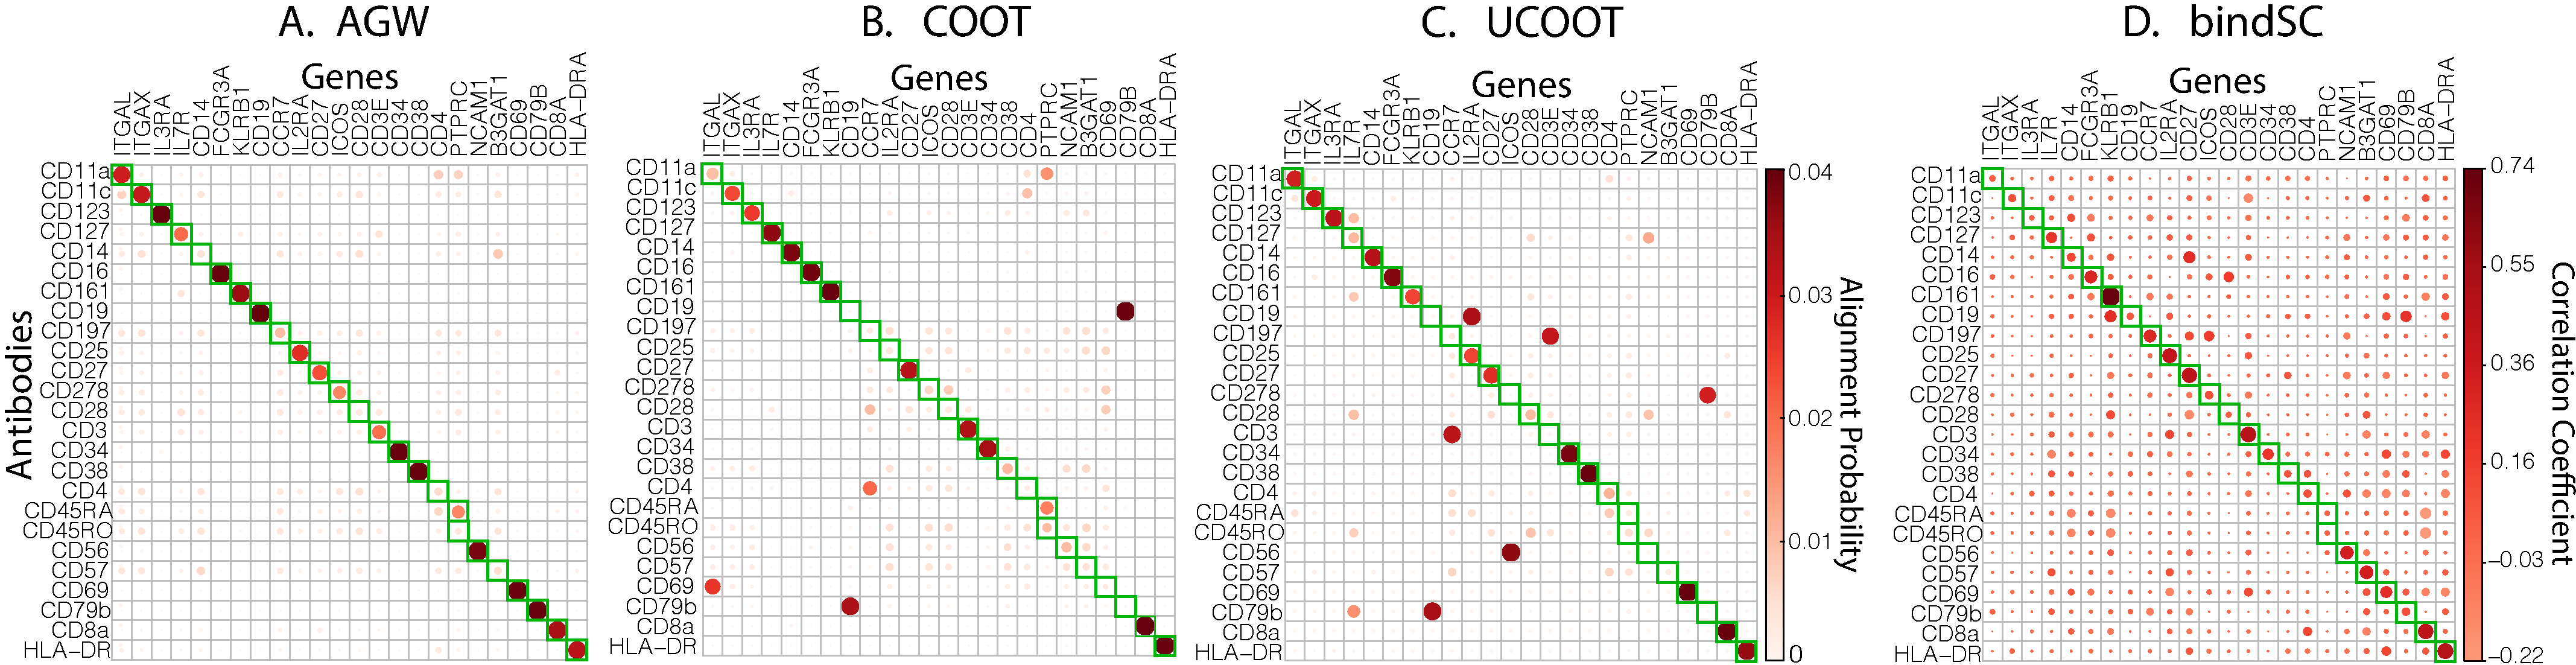
\includegraphics[width=\linewidth]{./Chapitre5/fig/cite_fgcoot_final.pdf}
\caption{\label{fig:cite} Feature alignments for the CITE-seq dataset. Green boxes indicate
where we expect matches (a notion of ``ground-truth'') based on domain knowledge.}
\label{}
\end{figure}

\subsection{Integrating single-cell multi-omics datasets}
Integrating data from different single-cell sequencing experiments is
an important biological task for which OT has proven useful \citep{Pamona,UniPort,Demetci20}.
Single-cell experiments measure various genomic features at the individual cell resolution.
Jointly studying these can give scientists insight into the mechanisms regulating cells.
However, experimentally combining multiple types of measurements for the same cell
is challenging for most combinations. Scientists rely on the computational integration
of multi-modal data taken on different but related cells (\textit{e.g.}, by cell type or tissue)
to study the relationships and interactions between different aspects of the genome.

We particularly focus on this task for two reasons. First, GW is used as a state-of-the-art
method for this task \citep{Pamona,Demetci22,UniPort}, so it is important to see if
AGW improves upon it. Second, several single-cell benchmark datasets provide
ground-truth matchings on the feature- and the sample-level alignments.
This information allows us to assess the effect of guiding cross-domain matching with partial
or full prior knowledge of these relationships.

\paragraph{Single-cell alignment} We follow the first GW application in this domain
\citep{Demetci20} and align samples (\textit{i.e.}, cells) of simulated and real-world datasets
from different measurement types. We have ground-truth information on cell-cell alignments
for all datasets, which we only use for benchmarking. We demonstrate in \Cref{table:scCells}
that AGW consistently yields higher quality cell alignments (with lower alignment error)
compared to the state-of-the-art baselines, including GW, COOT, and their unbalanced counterparts.

We include bindSC as an additional baseline, which performs bi-order canonical correlation analysis
to align single-cell datasets. Unlike other single-cell alignment methods,
it internally computes a feature correlation matrix that users can extract. So,
we include it as a baseline to compare its feature alignment performance against
AGW in the next section. However, bindSC usage is limited to a few measurement types
as it requires an input matrix that relates features across domains to bring the datasets
into the same space at initialization. We do not have this information for most datasets,
thus the ``N/A'' entries in \Cref{table:scCells}.

% It is important to note that an unbalanced extension could be developed for AGW through future work to potentially further boost the results.

\paragraph{Aligning genomic features} AGW augments GW formulation with a feature coupling matrix.
Therefore, we jointly align features and see whether AGW reveals relevant biological relationships.
All current single-cell alignment methods only align samples (\textit{i.e.}, cells),
except for bindSC as discussed above.

Among the real-world datasets in \Cref{table:scCells}, CITE-seq \citep{CITEseq}
is the only one with ground-truth information on feature correspondences.
This dataset has paired single-cell measurements on the abundance levels of
25 antibodies and activity (i.e., ``expression'') levels of genes,
including the genes that encode these 25 antibodies. So, we first present
unsupervised feature alignment results on the CITE-seq dataset. For completion,
we also report the biological relevance of our feature alignments on SNARE-seq \citep{SNAREseq}
and scGEM \citep{scGEM} datasets in Appendix Section 6.2.2. However, note that
these datasets (unlike CITE-seq) do not have clear ground-truth feature correspondences.
We compare our feature alignments with bindSC, COOT, and UCOOT in \Cref{fig:cite}.
The entries in the feature alignment matrices are arranged such that
the ``ground-truth'' correspondences lie in the diagonal, marked by green squares.
While AGW correctly assigns 19 out of 25 antibodies to their encoding genes with
the highest alignment probability, this number is 16 for UCOOT, 15 for COOT and
13 for bindSC (which yields correlation coefficients instead of alignment probabilities).
Additionally, the OT methods yield more sparse alignments thanks to
the ``least effort'' requirement in their formulation.

\begin{table*}[ht]
\caption{\label{tab:hda} \textbf{Heterogeneous domain adaptation results (unsupervised)}.
Best results are bolded, and second-bests are underlined. For AGW,
the $\alpha$ values used are respectively $0.6, 0.9, 0.7, 0.9, 0.3, 0.8, 0.7, 0.2, 0.6$. }
\begin{center}
\resizebox{1.0\linewidth}{!}{
\begin{tabular}{@{}lccccccccc@{}}
\toprule
               & \textbf{A $\rightarrow$ A} & \textbf{A $\rightarrow$ C} & \textbf{A $\rightarrow$ W} & \textbf{C $\rightarrow$ A} & \textbf{C $\rightarrow$ C} & \textbf{C $\rightarrow$ W} & \textbf{W $\rightarrow$ A} & \textbf{W $\rightarrow$ C} & \textbf{W $\rightarrow$ W} \\ \midrule


\textbf{AGW}   & \textbf{93.1$\pm$1.6}                               & \textbf{68.3$\pm$14.1}                              & \textbf{79.8$\pm$3.5}                               & \underline{55.4$\pm$7.1}                              & \underline{76.4$\pm$5.6}                               & \textbf{57.7$\pm$14.3}                              & 60.1$\pm$9.1                               & \textbf{60.9$\pm$13.3}                              & \textbf{97.3$\pm$0.9}                               \\
\textbf{GW}    & 86.2$\pm$2.3                               & 64.1$\pm$6.2                               & \underline{77.6$\pm$11.1}                              & 53.0$\pm$13.2                              & \textbf{81.9$\pm$10.5}                              & \underline{53.5$\pm$15.9}                              & 50.4$\pm$22.1                              & 54.3$\pm$14.7                              & 92.5$\pm$2.6                               \\
\textbf{COOT}  & 50.3$\pm$15.9                              & 35.0$\pm$6.4                               & 39.8$\pm$14.5                              & 40.8$\pm$15.8                              & 33.5$\pm$10.7                              & 37.5$\pm$10.4                              & 44.3$\pm$14.0                              & 27.4$\pm$10.2                              & 57.9$\pm$13.4                              \\
\textbf{UGW}   & \underline{90.6$\pm$6.5}                             & \underline{67.2$\pm$12.7}                            & 75.4$\pm$3.1                             & \textbf{56.3$\pm$14.6}                            & 69.2$\pm$8.7                            & 51.2$\pm$13.1                           & \textbf{66.7$\pm$9.9}                             & 58.4$\pm$4.7                            & \underline{94.7$\pm$1.5}                             \\
\textbf{UCOOT} & 65.4$\pm$2.1                              & 44.6$\pm$3.8                               & 36.4$\pm$1.2                               & 55.1$\pm$8.6                               & 52.1$\pm$3.8                               & 41.8$\pm$14.9                              & \underline{63.2$\pm$4.0}                               & \underline{59.7$\pm$6.3}                               & 80.3$\pm$2.1                               \\
\bottomrule
\end{tabular}}
\end{center}
\end{table*}

\paragraph{Leveraging prior knowledge}
Finally, we show the advantage of providing priors by aligning a
multi-species gene expression dataset containing measurements from
the adult mouse prefrontal cortex \citep{mouse} and pallium of bearded lizard \citep{lizard}.
Since measurements come from two different species, the feature space (i.e., genes) differs,
and there is no 1-1 correspondence between the samples (i.e., cells). However,
there is a shared subset within the features, i.e., orthologous genes that
descend from a common ancestor and maintain similar biological functions in both species.
We also have domain knowledge on cells that belong to similar cell types across the two species.
Thus, we expect AGW to recover these relationships.

\setlength{\columnsep}{10pt}%
\setlength{\intextsep}{0pt}
% \begin{wrapfigure}[15]{r}{\linewidth}
\begin{figure*}[!t]
\centering
\includegraphics[width=0.85\linewidth]{./Chapitre5/fig/xSp_full.png}
\caption{\label{fig:xsp} \textbf{Aligning cross-species dataset.}
A. AGW's cell-type alignments.
B. Providing supervision on one level of alignment (\textit{e.g.}, features)
boosts alignments on the other. Standard errors computed over 10 random runs.
Dashed line indicates the sample alignment performance of GW and bindSC
(orthologous gene used in input).}
\end{figure*}


% \begin{figure}
% \centering
% \includegraphics[width=0.8\linewidth]{figures/xSp_cellAlign.png}
% \caption{\textbf{Cell-type alignment results on cross-species dataset.}}
% \label{fig:crossAlignments}
% \end{figure}
%\end{wrapfigure}

\Cref{fig:xsp}A visualizes the cell-type alignment probabilities yielded by AGW
when full supervision is provided on the $10,816$ orthologous genes.
The green boxes indicate alignment between similar types of cells.
This matrix is obtained by averaging the sample alignment matrix
(\textit{i.e.}, cell-cell alignments) into cell-type groups. We observe that
AGW yields biologically plausible alignments, as all the six cell types that
have a natural match across the two species are correctly matched.
We also show in \Cref{fig:xsp}B that providing supervision on one alignment level (\textit{e.g.},
features) improves the quality on the other alignment level (\textit{e.g.}, samples).
The supervision scheme is detailed in Appendix Section 6.4.


\subsection{Heterogeneous domain adaptation}
Finally, we demonstrate the generalizability of our approach on a popular ML task,
heterogeneous domain adaptation, where COOT and GW were previously successfully used.
Domain adaptation (DA) refers to the problem in which a classifier learned on one domain
(called \textit{source}) can generalize to the other (called \textit{target}). Here,
we apply AGW to unsupervised and semi-supervised heterogeneous DA (HDA) tasks,
where the source and target samples live in different spaces, and we have as few as
zero labeled target samples.

We follow the experimental setup by \citep{Redko20} and use source-target pairs
from the Caltech-Office dataset \citep{Saenko10}. We consider all pairs between three domains:
Amazon (A), Caltech-$256$ (C), and Webcam (W), whose images are embeddings from
the second last layer in the GoogleNet \citep{Szegedy15} (vectors in $\bbR^{4096}$)
and CaffeNet \citep{Jia14} (vectors in $\bbR^{1024}$) neural network architectures.
In semi-supervised settings, we incorporate prior knowledge on a few target labels
by adding an extra cost matrix to the training of sample coupling, so that
a source sample will be penalized if it transfers mass to the target samples from different classes.
Once the sample coupling $P^s$ is learned, we obtain the final prediction using label propagation:
$\widehat{y}_t = \argmax_k L_{k\cdot}$,
where $L = D_s P^s$ and $D_s$ denotes one-hot encodings of the source labels $y_s$.
All hyperparameters are tuned on a validation set based on accuracy (Appendix ).

\Cref{tab:hda} presents the performance of each method averaged across ten runs in
the unsupervised setting, where AGW yields favorable results in 6 out of 9 cases. In two cases,
UGW, and in one case, UCOOT, outperform AGW despite the lower performance of
their balanced counterparts. In these cases, unbalanced formulations prove beneficial,
and support extending AGW to unbalanced scenarios as future work.
Appendix Section 6.4 presents the semi-supervised experiments,
which show the same trend where AGW tends to outperform other baselines.

In domain adaptation and transfer learning applications, the key is to perform
successful dataset comparisons. To more directly check if AGW yields improved object comparison,
we compute the correlation between AGW distance versus Optimal Transport Dataset Distance (OTDD)
\citep{Melis20}, an OT metric specifically developed to quantify dataset dissimilarities
for transfer learning applications. We replicate the original experiment comparing
USPS and MNIST datasets and three MNIST extensions: Fashion-MNIST, KMNIST, and EMNIST
(Appendix Section 6.4.3). AGW shows a Pearson's correlation of $>0.965$
with OTDD with p-value $<0.0001$ across varying levels of alpha, while for COOT, it is 0.7578
(p-value: 0.011), and for GW, -0.155 (p-value: 0.67).
This evaluation further supports that AGW interpolation leads to more informative dataset comparisons.
Note that AGW solely uses input data while OTDD also leverages labels when comparing datasets.

\paragraph{Empirical runtime} As described in Section 3.2,
the theoretical complexity of AGW is $O(n^3 + dn^2 + nd^2)$. When $d<n$,
the dominating term of $n^3$ is due to the computational burden of computing the GW distance.
However, in practice, we observe that AGW converges in much fewer iterations than GW
(about $1/5$ of the number of iterations on average) thus having a shorter runtime
(further detailed in Appendix Section 6.3). To further speed up optimization,
one can consider low-rank coupling and cost matrix \citep{Meyer21b} or
use the divide and conquer strategy \citep{Chowdhury21a},
which allows one to scale the GW distance up to a million points.

% Table 4 shows that AGW consistently performs well compared to the state-of-the-art baselines, which supports our claim about its capacity to properly adjust the invariance of the datasets at hand.

%except for the baseline, for each method, we use the learned sample coupling between source and  target data to predict the labels in the target domain via label propagation \citep{Redko19a}.
% More precisely, for each pair of domains, we randomly choose $20$ samples per class (thus $n_s = n_t = 200$) and
% perform adaptation from CaffeNet to GoogleNet features, then calculate the accuracy of the generated predictions on the target domain.
% We repeat this process $10$ times and calculate the average and standard deviation of the performance. Without prior knowledge, we assign uniform distributions to the samples and features in the source and target domains.

% Please add the following required packages to your document preamble:
% \usepackage{booktabs}



% \iffalse
% More precisely, we introduce the masked target label $\tilde{y}^{(t)} \in \bbR^{n_t}$
% defined by randomly keeping $\tilde{n}_t \in \{1,3,5\}$ samples in each class in the target label $y^{(t)}$ and masking all other
% labels in $y^{(t)}$ by $-1$. Then the additional cost $M \in \bbR^{n_s \times n_t}$ between $y^{(s)}$ and $\tilde{y}^{(t)}$ is defined by
% \begin{equation}
%   M_{ij} =
%   \begin{cases}
%     0, \text{ if } y^{(s)}_i = \tilde{y}^{(t)}_j, \text{ or } \tilde{y}^{(t)}_j = -1 \\
%     v, \text{ otherwise}.
%   \end{cases}
% \end{equation}
% Here, $v > 0$ is a fixed value and we choose $v = 100$ in this experiment.

% Once the sample coupling $P$ is learned, the label propagation works as follows:
% suppose the labels contain $K$ different classes,
% we apply the one-hot encoding to the source label $y^{(s)}$ to obtain
% $D^{(s)} \in \bbR^{K \times n_s}$ where $D^{(s)}_{ki} = 1_{\{y^{(s)}_i = k\}}$.
% The label proportions on the target data are estimated by: $L = D^{(s)} P \in \bbR^{K \times n_t}$.
% Then the prediction can be generated by choosing the
% label with the highest proportion, i.e. $\widehat{y}^{(t)}_j = \argmax_k L_{kj}$.

% Note that, while the prediction is performed on the whole target samples,
% only those whose labels are masked as $-1$ during the
% training, are used in the calculation of accuracy. For the $k$-NN only,
% we train a classifier on the labeled target samples,
% then perform prediction on the unlabelled ones.
% \fi

 %We also note that the naive choice of $\alpha=0.5$ already provides a strong baseline that improves
% \setlength{\tabcolsep}{8pt}



%first apply our formulation to three machine learning benchmarks. In the first, we
%and demonstrate that (1) the degree of invariant to local or global isometric transformations can be regulated through the proposed interpolation, as well as through prior information supplied on the feature coupling, and (2) different interpolation strenghs lead to

% {\color{red} This is a very rough first draft: I am jolting down some thoughts on how we could use the current experiments to sell the benefits of FGCOOT. -Pinar.}\\

% We show the following merits of \textsc{FGCOOT} through various experiments:
% \begin{itemize}
%     \item \textsc{FGCOOT} interpolates the two optimal transport distances that can be computed between datasets across different metric spaces, namely, \textsc{COOT} and \textsc{GW} \ref{Theorem1}. As these distances show .. We demonstrate through applications on hand-written digit alignment and heterogeneous domain adaptation tasks that in certain cases,
%     \item \textsc{FGCOOT}
% \end{itemize}

% \iffalse
% \subsection{Control over invariants}

% We observe that the interpolation
% Through two mechanisms: (1) interpolation between the GW and COOT terms (different coefficients of interpolation perform best for different cases -- HDA also demonstrates this), and (2)
% \begin{figure}[h]
% \centering
% \includegraphics[width=\linewidth]{figures/mnist1.png}
% \caption{\label{fig:mnist}\textbf{} }
% \end{figure}

% %\subsection{Heterogeneous domain adaptation}
% % Please add the following required packages to your document preamble:
% % \usepackage{booktabs}

% %\paragraph{Dataset} We consider the Caltech-Office dataset \citep{Saenko10} widely used in domain adaptation experiments. It contains three domains:  Amazon (A), Caltech-$256$ (C) and Webcam (W), whose images are embeddings extracted from the second last layer in the Google Net \citep{Szegedy15} (vectors in $\bbR^{4096}$) and Caffe Net \citep{Jia14} (vectors in $\bbR^{1024}$) neural network architectures.

% %\paragraph{Competing methods} We compare $2$ OT-based methods: GW, COOT. The details about the choice of hyperparameters  for each method can be found in the Appendix \ref{sec_app:exp}. For the semi-supervised HDA task, we use $k$-NN, with $k=3$ as baseline method, which corresponds to the situation where there is no adaptation.
% %\paragraph{Experimental setting}

% \subsection{Cross-domain imitation learning}
% In \citep{FickingerC0A22}, the authors used GW distance to solve a very challenging cross-domain imitation learning (IL) task. In general, the goal of IL is to learn a policy for an agent from expert state-action observations. In cross-domain setting, the agent additionally learns a different task in a different environment from that in which the expert operates. \citep{FickingerC0A22} proposed GWIL: an IL algorithm that uses GW distance between state-action pairs of the agent and the expert as a proxy for the reward that is then used in soft-actor critic (SAC) \citep{sac} algorithm to learn agent's policy. As our work intends to improve upon GW distance, below we provide the experimental results comparing our IL algorithm based on AGW to GWIL.

% \begin{wrapfigure}[15]{r}{.42\linewidth}
% \centering
% \includegraphics[width=.8\linewidth]{figures/rewards_vs_proxy_fgcoot_False_false_0.5.png}
%     \captionof{figure}{AGW values and true agents rewards for pendulum to cartpole task. AGW divergence exhibits a strong correlation with the true rewards.}
% \end{wrapfigure}


% \begin{table}
%     \centering
%     \caption{Best average reward attained by each method during evaluation.\label{tab:RL} }
%     \begin{tabular}{l|cc}
%        \textbf{Task}  &  \textbf{AGW} & \textbf{GWIL}\\
%        \hline
%        Pendulum $\rightarrow$ Cartpole & \textbf{187.47$\pm$10.05} & 109.66$\pm$ 2.7\\
%        Cheetah $\rightarrow$ Walker & \textbf{124.84$\pm$2.71} & 51.67$\pm$ 9.15
%     \end{tabular}

% \end{table}

% Following \citep{FickingerC0A22}, we consider two scenarios. First one is to learn agent's policy for cartpole swingup task from one demonstration of expert's state-action pairs for pendulum swingup task. Second is to learn a walker to walk from a demonstration of a running cheetah. As in \citep{FickingerC0A22}, we use simulated continuous control tasks implemented in Mujoco
% \citep{todorov} and the DeepMind control suite \citep{tassa}. For the first task, we use AGW with $\alpha=0.9$. We present the results for other values of $\alpha$ in the Supplementary materials. which favours GW term in our formulation. For the second task, we set $\alpha=0.5$ and run the evaluation over 3 seeds for the two scenarios. Table ~\ref{tab:RL} reports the highest average reward obtained by each method for both cases.


% Our results on the two cross-domain tasks show ...
% \fi

\section{Discussion and conclusion}

% We present Augmented Gromov-Wasserstein (AGW), a new OT-based divergence for incomparable spaces. AGW relies on the GW distance and CO-Optimal transport. This novel metric narrows down
We present Augmented Gromov-Wasserstein (AGW), a new OT-based divergence for incomparable spaces.
It interpolates between GW and CO-Optimal transport and allows to narrow down the
choices of isometries induced by GW, while efficiently exploiting the prior knowledge
on the input data. We study its basic properties and empirically show that such restrictions
result in better performance for single-cell multi-omic alignment tasks and transfer learning.
Future work will focus on refining the theoretical analysis of the AGW invariants to
better understand their performance in practice. We will also extend AGW to the unbalanced
and/or continuous setting, and other tasks where feature supervision by domain experts
may be incorporated in OT framework.

